\chapter{Analysis and Results}
\label{cha:results}

In this chapter the implementation of the SMS Analysis/Synthesis system done in MATLAB is analyzed for performance and the results are presented.

The aim of this auralization approach was to generate perceptually similar sounds, which are not necessarily mathematically similar. Thus, simple numerical comparisons might not yield much information of the ability of the system to model and auralize the sounds. Nonetheless, energy analysis and spectral comparisons can be used to get a basic understanding of the success of the auralization.

A perceptual test can give a better indication of the ability of the system to synthesize the sounds well. Hence, a listening test was also performed using external participants to compare sounds and gauge the performance of the auralization.

%%%%%%%%%%%%%%%%%%%%%%%%%%%%%%%%%%%%%%%%%%%%%%%%%%%%%
\section{Numerical Results}
\label{sec:num_res}

\subsection{Energy Analysis}
\label{sec:energy_analysis_results}

Energy analysis, which is a form of numerical analysis, was performed at various stages of the Analysis/Synthesis system. As explained in section \ref{sec:energy_analysis}, the flow of energy through the various components of the model is critical in understanding the working of SMS technique. For the analysis of this method, energy analysis was performed in sections, before and after many intermediate steps, calculating the total energy before and after each step. Table \ref{tab:energy_table} shows the energy analysis between various steps for an example analysis done on a recording of the King Long Bus driving at 90kmph. While the units of energy calculated is arbitrary using Eq. .\ref{eqn:parsevals}, the comparison between the values gives an idea of the flow of energy during the entire modeling process.

A few interesting patterns can be see from these values. Before the energy thresholding process, the peak trajectories track a lot more energy than there exists in the original sound. This is due to the interpolation and amplitude smoothing (sleeping and removal of small sleep durations) functionality of the trajectories. This also proves that the trajectory-tracking algorithm tends to track peaks that might not be tones but just peaks generated by higher noise energy in that frequency for that frame and assumes them as being tones. The energy threshold filter however does help to reduce a large part of these inaccurately tracked trajectories.

Another observation is that some energy seems to have been lost in the removal of the deterministic signal from the original signal in order to generate the Residual signal. The can be attributed to the method used in spectral subtraction where the magnitude is not allowed to reduce below zero even if the deterministic spectrum has higher magnitude than the spectrum of the original signal in the same frequency bin.

Finally, the total energy level at the end of the synthesis is also about 10\% less than the energy at the beginning. This difference is the most important metrics that has to be analyzed. While the nature of the modeling process definitely causes the energy to be lost in the various stages, a number which is significantly close to the original value is critical in ensuring that model was accurate in capturing the important aspects of the sound. However, differences in the energy levels do not indicate a definite perceptual difference in the sounds, but they do indicate a possibility of such a difference.

Finally, the difference in the original and re-synthesized sound energy levels means that the perceived loudness of the two sounds might be different. This has to be taken into account when designing the listening tests in Section \ref{sec:listeningTests}. For the listening tests, the re-synthesized sound has to be scaled to have the same energy as the original to ensure similar loudness levels.

\begin{table}[ht]
\begin{center}
\begin{tabular}{| l | c |}
  \hline
  Sound & Energy [dB re-arbitary] \\ \hline \hline
  Original Sound & 78.359 \\  \hline
  Peak Trajectories (before Energy Tresholding)& 85.553 \\
  Peak Trajectories (after Energy Tresholding)& 38.3 \\
  Residual & 28.53 \\
  Parameterized Residual  & 30.102 \\
  Parameterized Residual (after Parameter Smoothing)  & 29.787 \\
  Re-Synthesied Tones & 38.3 \\
  Re-Synthesized Noise & 29.487 \\
  Re-Synthesized Combined Sound & 66.548 \\
  Re-Synthesized Combined Sound (Energy Scaled) & 78.359 \\ \hline
\end{tabular}
\caption{Energy values in arbitrary units before and after each step of the SMS process normalized to the original energy.}
\label{tab:energy_table}
\end{center}
\end{table}

%%%%%%%%%%%%%%%%%%%%%%%%%%%%%%%%%%%%%%%%%%%%%%%%%%%%%
\subsection{Spectral Comparison}
\label{sec:realtime}

While energy analysis gives an idea of net energy levels in the various components of the modeling technique, a spectral comparison allows a visual inspection of the differences between the original sound and re-synthesized sound. The MATLAB \emph{spectrogram} function can be used to plot spectrograms of the original sound and re-synthesized sound for comparison. Figures \ref{fig:spec_comp1}-\ref{fig:spec_comp3} shows a few of the sounds which have been re-synthesized based on the source data.

\begin{figure}[!ht]
\begin{center}
\subfigure[Original]{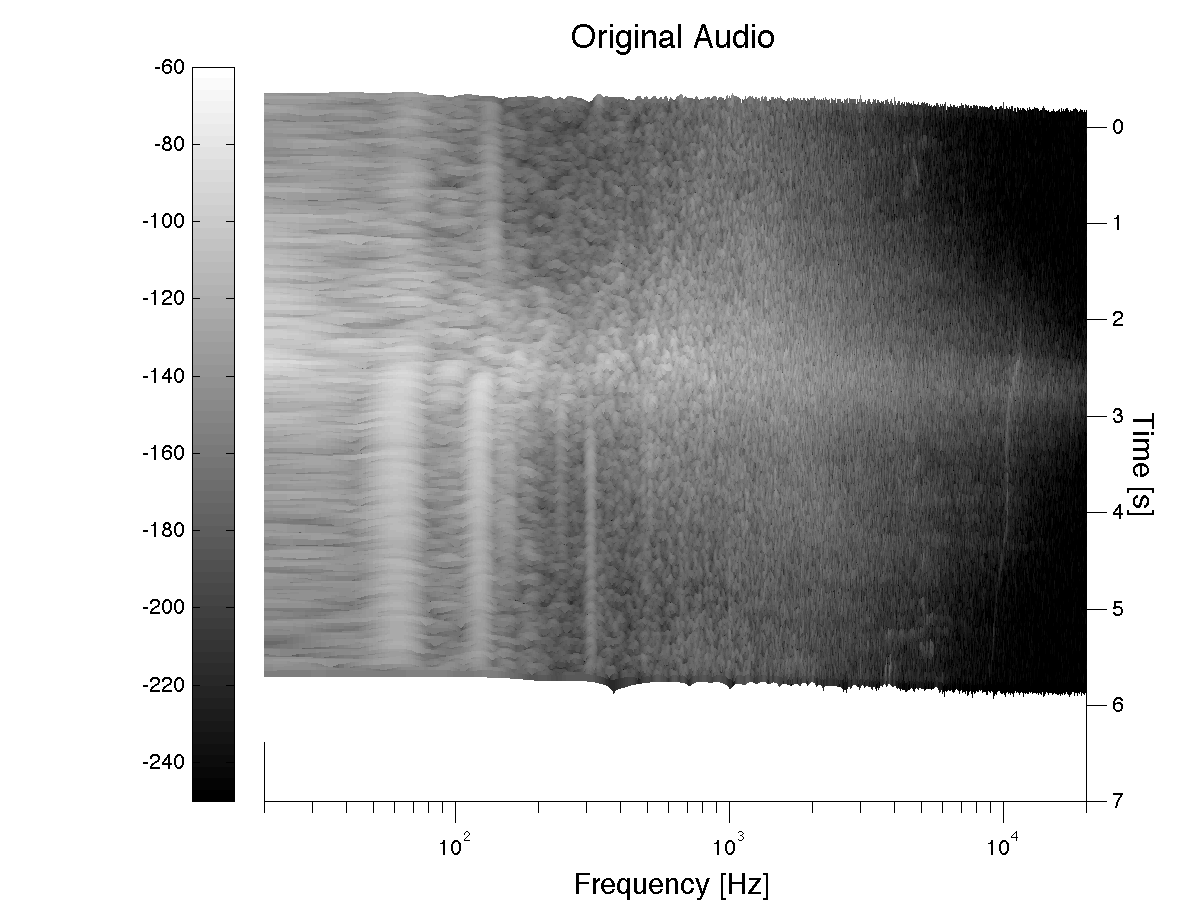
\includegraphics[height=5.2cm]{../images/spec_orig1.png}}
\subfigure[Re-Synthesized]{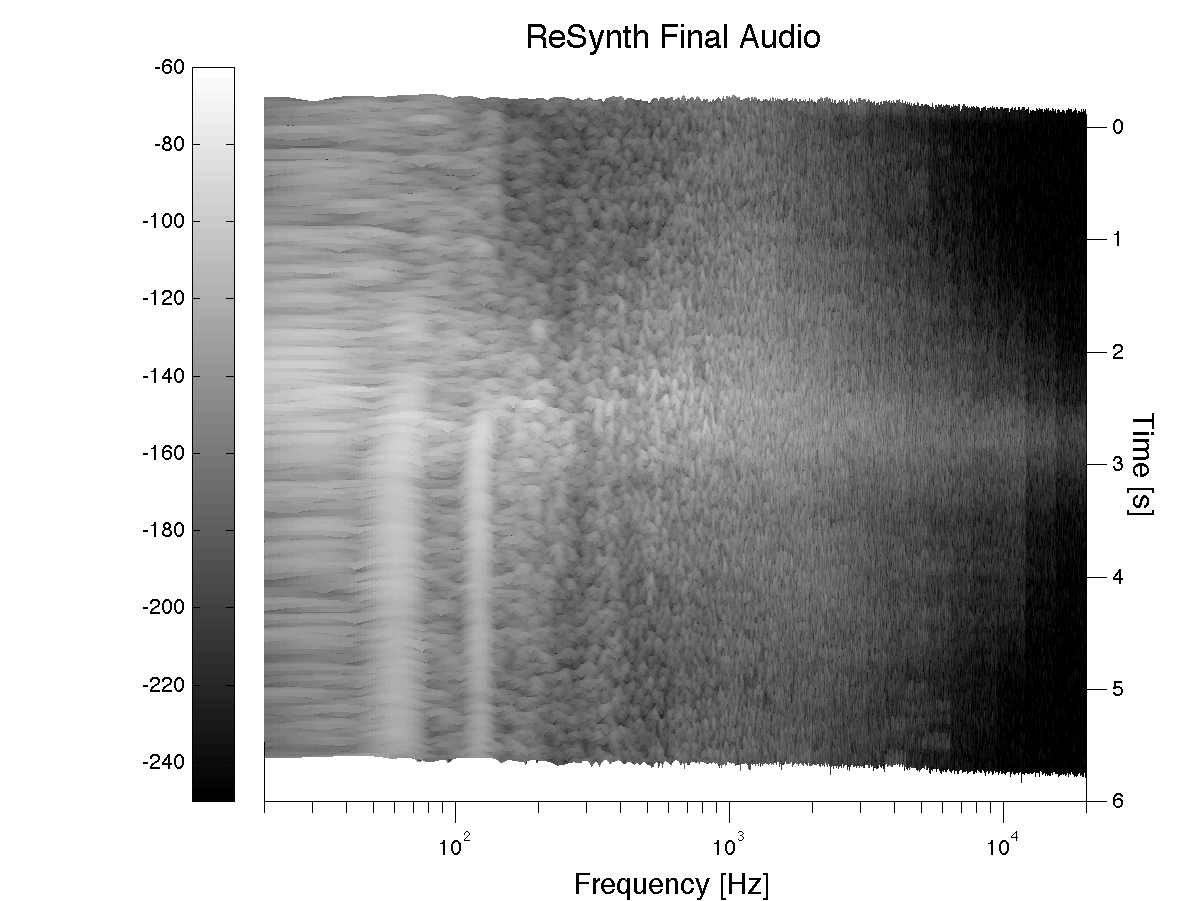
\includegraphics[height=5.2cm]{../images/spec_resynth1.png}}
\caption{Spectrogram Comparisons of a passage of a King Long bus at 90kmph.}
\label{fig:spec_comp1}
\end{center}
\end{figure}

\begin{figure}[!ht]
\begin{center}
\subfigure[Original]{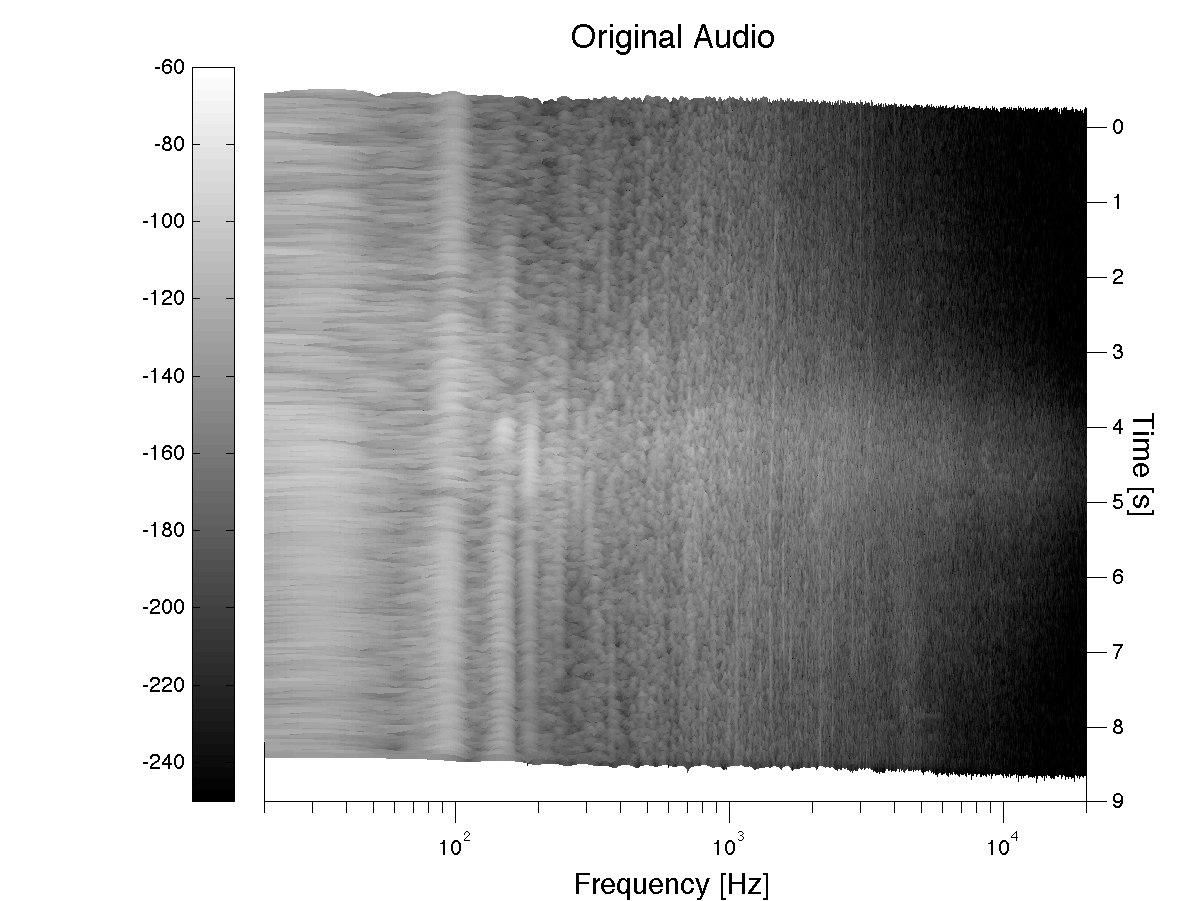
\includegraphics[height=5.2cm]{../images/spec_orig2}}
\subfigure[Re-Synthesized]{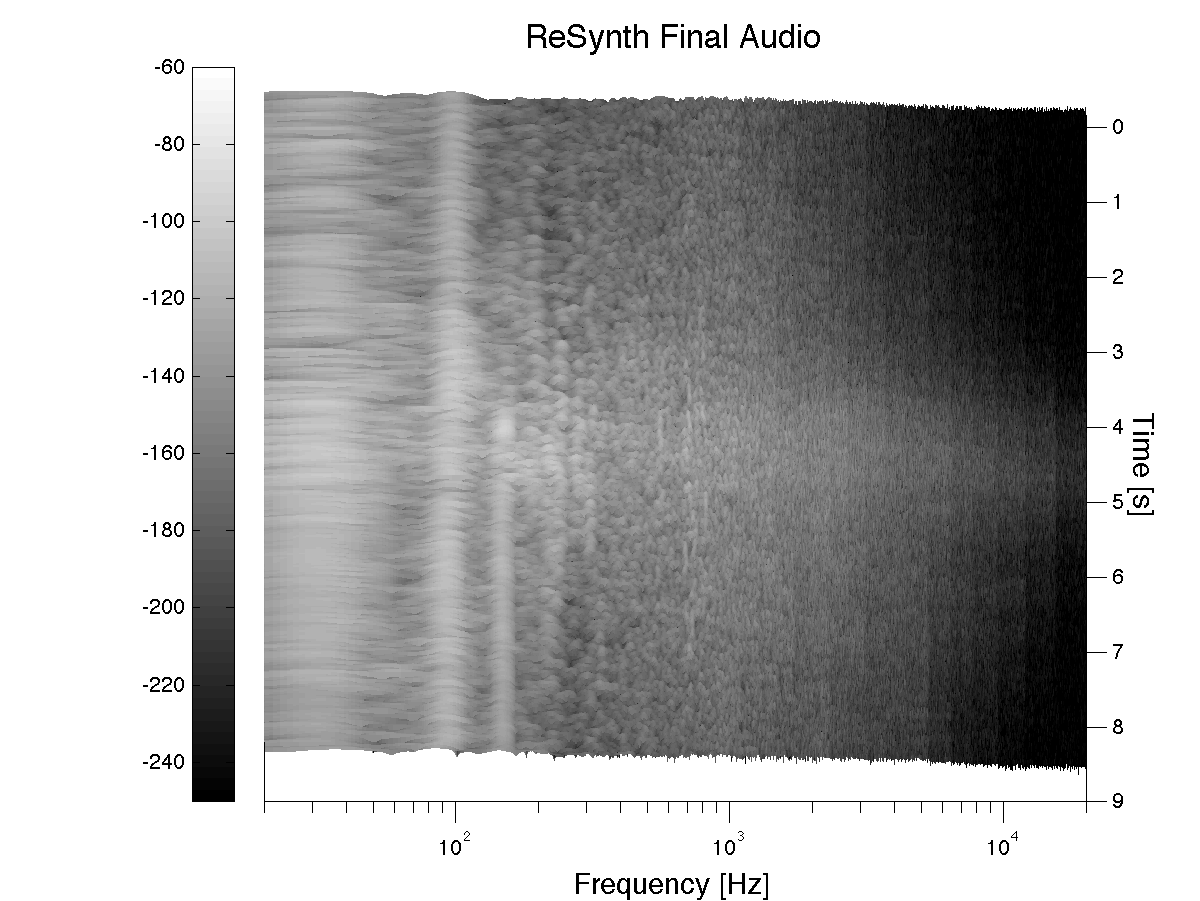
\includegraphics[height=5.2cm]{../images/spec_resynth2}}
\caption{Spectrogram Comparisons of a passage of a King Long bus at 30kmph.}
\label{fig:spec_comp2}
\end{center}
\end{figure}

\begin{figure}[!ht]
\begin{center}
\subfigure[Original]{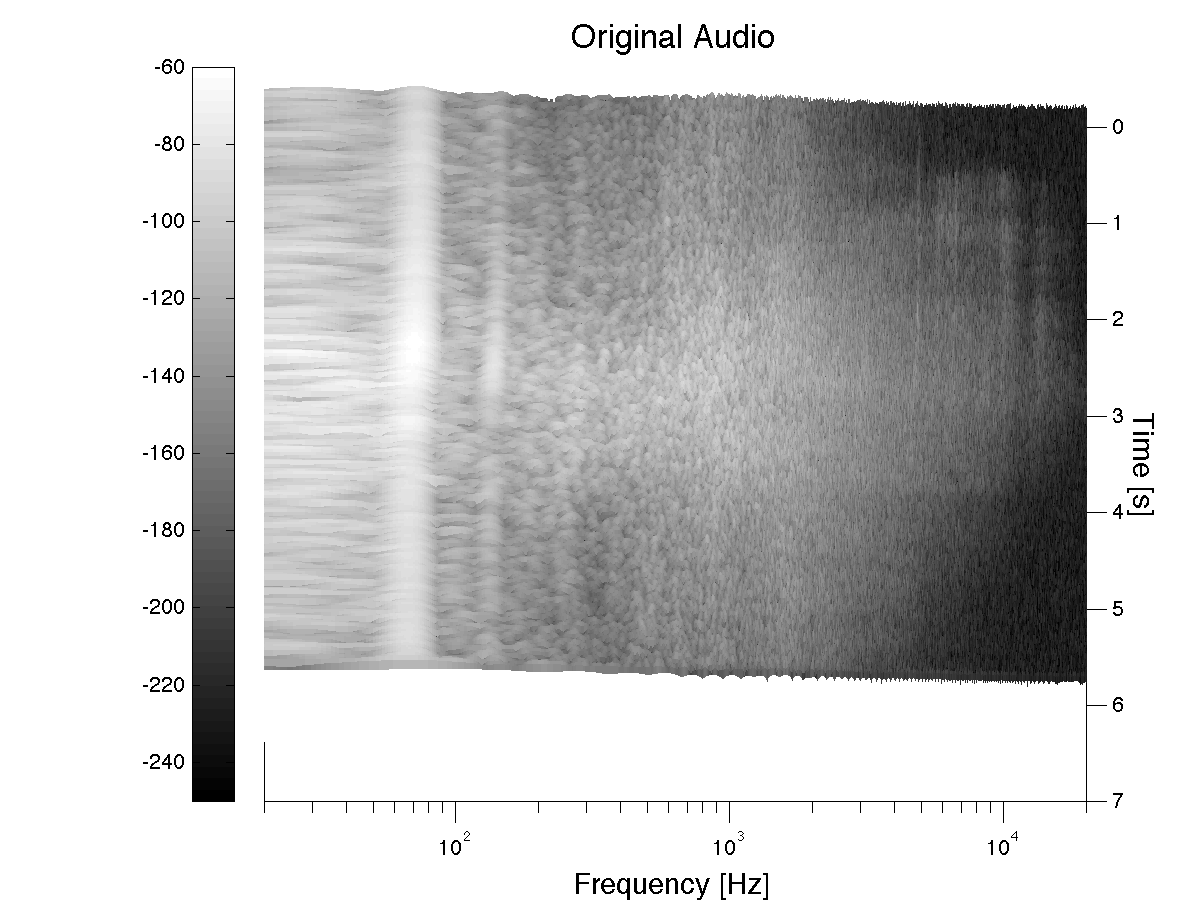
\includegraphics[height=5.2cm]{../images/spec_orig3}}
\subfigure[Re-Synthesized]{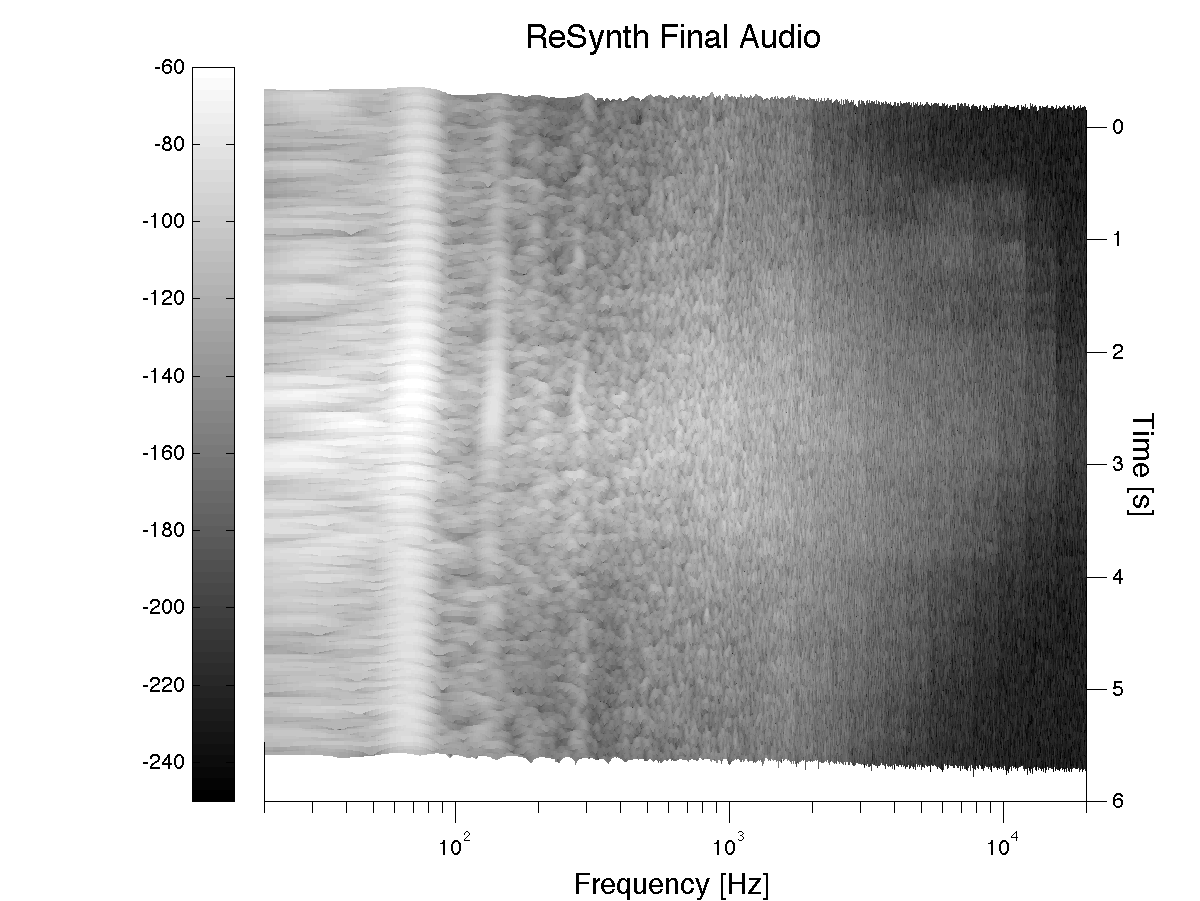
\includegraphics[height=5.2cm]{../images/spec_resynth3}}
\caption{Spectrogram Comparisons of a passage of a Iveco Medium Heavy at 40kmph.}
\label{fig:spec_comp3}
\end{center}
\end{figure}

Three inferences can be drawn from the spectral comparison. A large portion of the low frequency content is modeled well by the peak tracking component of the algorithm, however, many redundant peaks are also tracked and generated into trajectories by the algorithm. These might not be audible when heard along side the other trajectories and the noise, because of their low amplitude. Hence the tracking and modeling of these peaks is redundant and should be avoided.

The parametrization of the noise into critical bands generates noise with very specific band edges visible in the noise amplitude. Such edges should not affect the sound perceptually \cite{ref:goodwin}, but the bands are visible in the spectrogram. Furthermore, synthesized Gaussian noise that has much greater amplitudes than the original uniform noise, which is noticeable in the spectrogram. However, as discussed in Section \ref{sec:equiEnergy}, the amplitude does not affect the auditory perception of noise as opposed to the total energy of the noise in that frequency band, which has been kept constant in the SMS process.

The balance between the tonal component and noise component has been kept through the Analysis/Synthesis process especially with the addition of the Energy scaling as explained in Section \ref{sec:energyscaling}. This is critical to have a good perception of the vehicle sound. While it is harder to see this comparison in the energy analysis, the levels of the spectrogram of the re-synthesized sound are similar to the original sound. This can be confirmed in the listening test results as well.

%%%%%%%%%%%%%%%%%%%%%%%%%%%%%%%%%%%%%%%%%%%%%%%%%%%%%
\section{Listening Tests}
\label{sec:listeningTests}

To analyze the ability of the implemented SMS system to auralize sounds, a listening test was conducted to test the perceptual fidelity of the re-synthesized sound. The aim of the test was to know if the original and re-synthesized sounds were significantly different when heard by humans.

\subsection{Test Design}

Since the entire test revolves around comparison of the original and re-synthesized sound, a matched pair test \cite{ref:matchPairTesting} was chosen to compare the two sound.

A matched pair test exposes the subjects to a sound pattern with a pair of sounds and allows them to choose one of the pair based on some criteria. The results are then tabulated to look at how many participants choose which of the two sounds in each of the pairs. It can be hypothesized that if the sounds are perceptually similar, the participants would not be able to tell the difference and hence choose both the original or re-synthesized sound with equal probability. Hence a matched pair difference test will tell us if the difference between the choice of either original or re-synthesized sound over the other is significant or not.

Selecting the original and corresponding re-synthesized sounds together and concatenating them one after each other generated the test sound patterns. A total of 18 original sounds were chosen based on the available recordings of the various vehicles. Table \ref{tab:sounds_table} shows the sounds used for the listening test.

\begin{table}[ht]
\begin{center}
\begin{tabular}{| c | l | l | c |}
\hline
& Filename & Vehicle Type & Speed (kmph)\\
\hline
1 & s\_otto34\_v45kmph.wav & Opel Astra & 45 \\
2 & vd\_30\_vx2\_6s-trimmed.wav  & Volvo V70 & 30\\
3 & vd\_50\_vx4\_6s-trimmed.wav  & Volvo V70 & 50\\
4 & vd\_70\_vx5\_6s-trimmed.wav  & Volvo V70 & 70\\
5 & vd\_90\_vx5\_6s-trimmed.wav  & Volvo V70 & 90\\
6 & iv\_20\_vx2\_6s-trimmed.wav & Iveco Medium Heavy & 20\\
7 & iv\_31\_vx3\_6s-trimmed.wav & Iveco Medium Heavy & 31\\
8 & iv\_40\_vx3\_6s-trimmed.wav & Iveco Medium Heavy & 40\\
9 & iv\_50\_vx4\_6s-trimmed.wav & Iveco Medium Heavy & 50\\
10 & iv\_70\_vx5\_6s-trimmed.wav & Iveco Medium Heavy & 70\\
11 & buss\_21\_gear2\_cal-trimmed.wav & King Long Bus &  21\\
12 & buss\_22\_gear2\_cal-trimmed.wav & King Long Bus &  22\\
13 & buss\_30\_gear3\_cal-trimmed.wav & King Long Bus &  30\\
14 & buss\_39\_gear4\_cal-trimmed.wav & King Long Bus &  39\\
15 & buss\_48\_gear5\_cal-trimmed.wav & King Long Bus &  48\\
16 & buss\_70\_gear7\_cal-trimmed.wav & King Long Bus &  70\\
17 & buss\_86\_gear7\_cal-trimmed.wav & King Long Bus &  86\\
18 & buss\_91\_gear8\_cal-trimmed.wav & King Long Bus &  91\\
\hline
\end{tabular}
\caption{Sounds used in the listening test.}
\label{tab:sounds_table}
\end{center}
\end{table}

Since the sounds were of vehicle passing by, all the sounds were edited such that the point of passage was exactly at the midpoint of length of the audio. The sounds were also trimmed to a duration 5 s before being analyzed and synthesized. The duration of 5 s was chosen to ensure that participants were able to recall the first sound in the test while the second sound was being played to be able to compare the sounds \cite{ref:Mats}. As explained in Section \ref{sec:energy_analysis_results} there was a difference in the total energy levels between the original and the re-synthesized sound. This was perceived as a difference in the loudness of the sounds. Hence to ensure that such factors do not affect the listening test, the re-synthesized sound was scaled to ensure that it has the same energy level as the original sound and thus a similar loudness level as described in Section \ref{sec:energyscaling}.

Table \ref{tab:sms_listening_test_params} in Appendix \ref{apd:ltest_data} shows the SMS parameters used for the analysis and synthesis for the listening test.

The original and re-synthesized sounds were concatenated to make a test pattern. A silence of 0.5 s was added before the first sound as well as between the two sounds to allow the participants to distinguish them. After the second sound, a pause of 4 seconds was added to ensure that the participants had enough time to answer the question.

The sounds were categorized by the four types of vehicles. Since the light vehicles have softer sounds, and the heavier vehicles have louder sounds, the patterns were played back according to categories from the light to heavy vehicles, so as to avoid the listener�s ears from being unable to perceive softer sounds after hearing loud sounds.

The sound patterns were generated in both orders, with the original sound being played first (AB) and it being played second (BA). This was to reduce the effect of bias towards the play order of individual sounds in a pattern. Furthermore, each order of pattern was played twice to reduce the effect of bias towards the play order within each category. Thus, each pair was played 4 times, within a section of the listening test. Thus, 72 sound patterns were created per criteria.

Table \ref{tab:sound_order} in Appendix \ref{apd:ltest_data} shows the order of pairs of sounds played during the listening test.

Three questions were asked as a criterion for the choice between two sounds. These questions tested the three most important aspects of the vehicle sound that need to be reflected in the synthesis. The realism of the re-synthesized sounds is important to make the listener believe that they is listening to the actual vehicle. The perceived annoyance factor of the vehicles is critical as it is most often the big aspect of decision making in soundscape design and thus, has to be tested to be similar between the original and re-synthesized. Finally the perceived speed of the vehicles is an important which affects annoyance as well and hence is also a factor in the decision making process. Thus the questions listed in Table \ref{tab:test_questions} were used in the test.

\begin{table}[ht]
\begin{center}
\begin{tabular}{| c | l | c |}
\hline
Section & Question & Number of Sound Pairs\\
\hline
1 & Which of the two sounds is a real recording? & 72\\
2 & Which of the two sounds is more annoying? & 72\\
3 & In which sound is the vehicle moving faster? & 72\\
\hline
\end{tabular}
\caption{Questions asked in the listening test.}
\label{tab:test_questions}
\end{center}
\end{table}

\subsection{Statistics}
\label{sec:stats}

A test comparing two things is statistically modeled as a match pair difference t-test. This test decides of there is significant difference between the choices of either one of the sounds. In the case of the listening test, since the aim is to find if there is any difference in the choice of the sounds, regardless if it�s favouring the original or the re-synthesized, a two-tailed test has to be performed.

For this test, our null hypothesis, $H_0$, is that there is $\mu_d= 0$, where $\mu_d$ is the true difference between the number of time a sound was chosen in the specific pair by the population. And thus our alternative hypothesis, $H_1$, is $\mu_d \not= 0$.  Thus, our null hypothesis states that the expected number of times either of the sounds is chosen, is equal. The test shall be done at 90\% confidence level, which is sufficient for such an application.

\subsection{Listening Test Implementation}

The listening test was carried out between 7th September and the 17th of September 2011 at the Division of Applied Acoustics, at Chalmers University of Technology, teaching lab. The participants were tested in groups of 1 to 7 at a time. The participants listened to the list of 72 combinations of the pairs for each of the three questions and answered which of the two sounds answered the question more aptly. The answers were shaded into circles of an optical marking sheet. The participants were given a 5 minute break between each question and the corresponding set of 72 sound patterns. The participants listened to the sounds on a pair of Sennheiser HD414 open back headphones along with a sub woofer that enhanced the lower frequencies. Two separate NAD 3020 amplifiers through a M-Audio Mobile Pre USB audio interface fed both headphones and sub woofer. The headphones and the sub woofer were calibrated to give a sound level of 94 dB at the listener position for a sound being played which was -6 dB from the maximum digital sound level. A total of 28 participants were tested, out of which 21 sets of completely valid data was gathered.

\subsection{Listening Test Results}

Figure \ref{fig:list_test_results} shows a summary of the average results of the listening test. For each sound, the graph compares the percentage of pairs where the original sound was chosen by the participants to answer the criteria. A result of 50 \% would indicate that both  sounds were chosen equally often, implying the inability of the participants to make any difference between the sounds with respect to the criteria.

\begin{figure}[ht]
\begin{center}
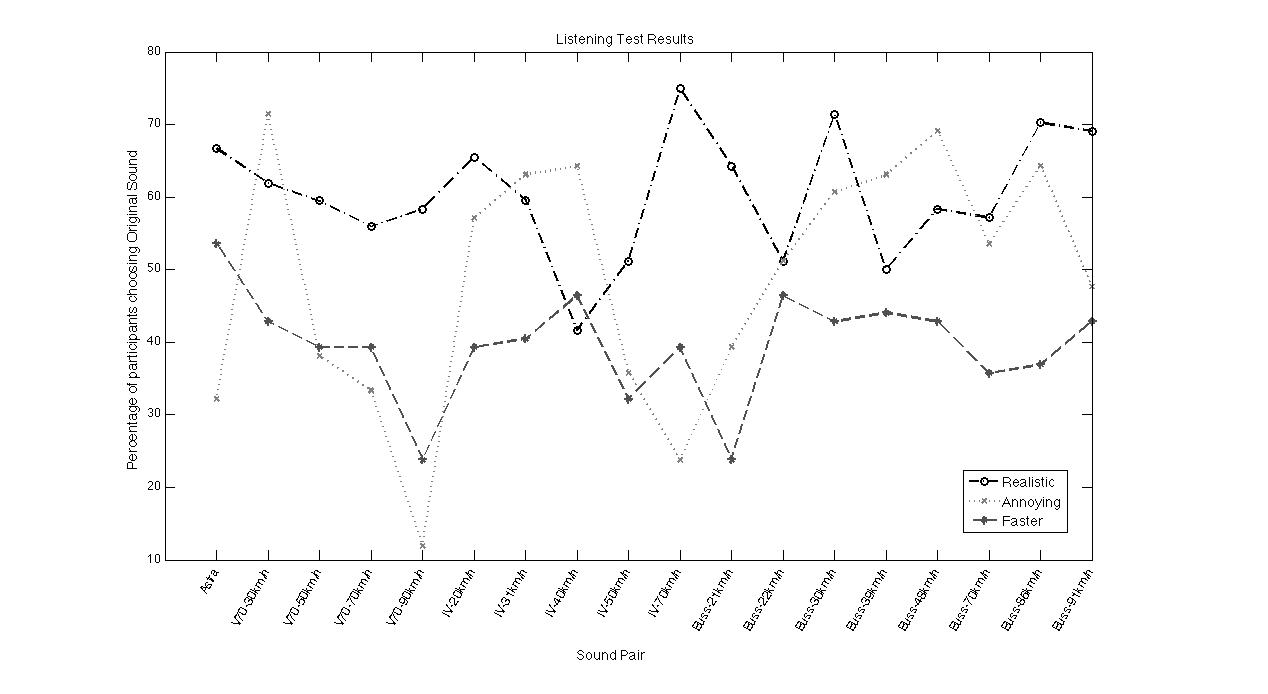
\includegraphics[height=8cm]{../images/prelimResults}
\caption{Summary of average results from the listening test.}
\end{center}
\label{fig:list_test_results}
\end{figure}

Considering the criteria of realism, a tendency can be observed towards the choice of the original sound, indicating a slight awareness and differentiability of the sound. Similar with speed, the tendency towards the re-synthesized sounds indicates that the perception of the speed of the vehicles in the re-synthesized sounds is greater. With annoyance, not much inferred, although it seems that the re-synthesized version of the pass-by of V70-90 was considered to be annoying by a large number of participants, possibly indicating a specific issue with the synthesis of that sound.

The plot gives a general idea of the perception of the re-synthesized sounds, but a statistical significance test has to be done to be able to claim the lack of significance in the differentiability of the two sounds.

\subsection{Statistical t-test}

Based on the matched pair t-test setup as described in Section \ref{sec:stats}, the test statistic for each pair can be calculated. An example for a specific sound (King Long Bus traveling at 70kmph) is shown in Table \ref{tab:ttest_diff}.

\begin{table}[ht]
\begin{center}
\begin{tabular}{| c | c | c | c | l |}
\hline
Listener & Original & Re-Synthesized & Difference, d & $\left(d - \overline{d} \right)^2$ \\
\hline
1 & 1 & 3 & -2 & 6.61 \\
2 & 0 & 4 & -4 & 20.90 \\
3 & 4 & 0 & 4 & 11.76 \\
4 & 4 & 0 & 4 & 11.76 \\
5 & 3 & 1 & 2 & 2.04 \\
6 & 2 & 2 & 0 & 0.33 \\
7 & 1 & 3 & -2 & 6.61 \\
8 & 4 & 0 & 4 & 11.76 \\
9 & 2 & 2 & 0 & 0.33 \\
10 & 2 & 2 & 0 & 0.33 \\
11 & 3 & 1 & 2 & 2.04 \\
12 & 1 & 3 & -2 & 6.61 \\
13 & 3 & 1 & 2 & 2.04 \\
14 & 4 & 0 & 4 & 11.76 \\
15 & 3 & 1 & 2 & 2.04 \\
16 & 3 & 1 & 2 & 2.04 \\
17 & 1 & 3 & -2 & 6.61 \\
18 & 2 & 2 & 0 & 0.33 \\
19 & 4 & 0 & 4 & 11.76 \\
20 & 0 & 4 & -4 & 20.90 \\
21 & 1 & 3 & -2 & 6.61 \\
\hline
\end{tabular}
\caption{Calculation for T-Test for the sound pair of the King Long Bus traveling at 70kmph for the question of realism of the sound.}
\label{tab:ttest_diff}
\end{center}
\end{table}

Firstly, a new variable, $d$ can be defined to indicate the difference between the paired values. In this case, it would be the difference between the number of times a original or re-synthesized sound was choosen. Eq. \ref{eq:ttestsetup} defines this,

\begin{equation}
\label{eq:ttestsetup}
d_i = n_{i,orignal} - n_{i,re-synthesized}
\end{equation}

where $n_{i,orignal}$ is the number of times the original version of a specific sound was chosen by the $i^{th}$ participant and $n_{i,re-synthesized}$ is the number of times a specific sound was chosen by the $i^{th}$ participant.

Next, the sample mean, $ \overline{d}$ of the differences is calculated as per Eq. \ref{eq:ttestsamplemean},

\begin{equation}
\label{eq:ttestsamplemean}
 \overline{d} = frac{(\sum_{i} d_i)}{n}
\end{equation}

where $n$ is the total number of participants.

Next, the standard deviation of the sample is calculated based on Eq. \ref{eq:std_dev}:

\begin{equation}
\label{eq:std_dev}
s_d = \sqrt{\frac{ \sum(d_i - \overline{d})^2}{  (n - 1)}}
\end{equation}

Based on the standard deviation, a standard error of the entire population can be estimated. In the case of the population, $N$, being much larger $(N >> n)$ than the sample size, $n$, Eq. \ref{eq:std_err} can be used as an estimate of the standard error :

\begin{equation}
\label{eq:std_err}
SE = \frac{s_d}{\sqrt(n)}
\end{equation}

Hence the test statistic can be expressed as:

\begin{equation}
\label{eq:test_stat}
t = \frac{(\overline{x}_1-\overline{x}_2)-D}{SE} = \frac{\overline{d}-D}{SE}
\end{equation}

where $D$ is the hypothesized mean difference between the population pairs, which in the case of the null hypothesis is 0.

Looking up the test statistic at significance level in the t-distribution gives p-value of the t-statistic. If the p-value is greater than the significance level, then it can be concluded that the null hypothesis cannot be rejected.

MATLAB also provides a method, \emph{ttest}, which automates the calculation of the test results. Running it on the results from the listening test gives the acceptance or rejection of the null hypothesis. In the cases of the acceptance, a conclusion can be drawn that for that specific criteria, there is no significant difference in the original and re-synthesized sounds. For the rejected cases, the conclusion has to be drawn that there is significant difference that the participants are able to detect. Table \ref{tab:ttest_results} tabulates the results of the t-test. Overall, the null hypothesis had to be rejected $30$ times, while it was accepted $24$ times.


\begin{table}[ht]
\begin{center}
\begin{tabular}{| c | l | c | l | l | l |}
\hline
Pair & Vehicle & Speed (kmph) & Realism & Annoyance & Speed \\
\hline
1 & Opel Astra & 45 & Rejected & Rejected & Accepted \\
2 & Volvo V70 & 30 & Rejected & Rejected & Accepted \\
3 & Volvo V70 & 50 & Rejected & Rejected & Rejected \\
4 & Volvo V70 & 70 & Accepted & Rejected & Accepted \\
5 & Volvo V70 & 90 & Accepted & Rejected & Rejected \\
6 & Medium Heavy & 20 & Rejected & Accepted & Rejected \\
7 & Medium Heavy & 31 & Accepted & Rejected & Rejected \\
8 & Medium Heavy & 40 & Accepted & Rejected & Accepted \\
9 & Medium Heavy & 50 & Accepted & Rejected & Rejected \\
10 & Medium Heavy & 70 & Rejected & Rejected & Accepted \\
11 & Bus &  21  & Rejected & Accepted & Rejected \\
12 & Bus &  22 & Accepted & Accepted & Accepted \\
13 & Bus &  30 & Rejected & Rejected & Accepted \\
14 & Bus &  39 & Accepted & Rejected & Accepted \\
15 & Bus &  48 & Accepted & Rejected & Accepted \\
16 & Bus &  70 & Accepted & Accepted & Rejected \\
17 & Bus &  86 & Rejected & Rejected & Rejected \\
18 & Bus &  91 & Rejected & Accepted & Accepted \\
\hline
\end{tabular}
\caption{Results of the t-test for significant difference on the listening test sounds.}
\label{tab:ttest_results}
\end{center}
\end{table}